\section{Results}

\begin{slide}
    Longevity-Based Batching
     \begin{itemize}
         \item {\sl Can batching based on longevity recognize fine/coarse parallelism in an application?}
        \item[] ~
    \end{itemize}

    Channel Pinning 
    \begin{itemize}
        \item {\sl Can an {\em even}-like spread increase early saturation?}
        \item[] ~
    \end{itemize}

    Bipartite-Graph Aided Sorting
    \begin{itemize}
        \item {\sl Are alternate channel implementations worth exploration?}
    \end{itemize}

    \inote{
        \item Remind about the goals of the talk. 
        \item LBB: Would like to take advantage of the frequency of communication. 
            
    }
\end{slide}

\begin{slide}
\frametitle{Results: Longevity-Based Batching}

        \begin{table}[htp!]
            \centering
            \begin{tabular}{@{}cccc}
                & \multicolumn{3}{c}{$PRing_N$} \\ \cline{2-4}
            & $N=P=8$ & $N=B=10$ & $N=2*B=20$     \\ \cline{2-4} 
                \multicolumn{1}{c|}{\rotatebox{90}{\rlap{\textbf{Reduc. Density}}}} & 
            \multicolumn{1}{c|}{\includegraphics[scale=0.15]{tests/pring/longbatcher/8/pg_0004.pdf}} & 
            \multicolumn{1}{c|}{\includegraphics[scale=0.15]{tests/pring/longbatcher/10/pg_0004.pdf}} & 
            \multicolumn{1}{c|}{\includegraphics[scale=0.15]{tests/pring/longbatcher/20/pg_0004.pdf}} \\ 
            \cline{2-4} 
        \end{tabular}
        \caption{Comparison of different sized $PRing_N$ on the Longevity 
                 Batching Scheduler with batch size $B=10$.}
            \label{tab:pring-longbatcher-testing}
        \end{table}

    \inote{
        \item Early tests gave promising results. 

        \item Here is $PRing_N$ which shows the reabsorption and containment on a single LPU as expected and hoped.

        \item So does batching based on longevity really recognize fine/coarse parallelism in an application?

        \item Sort of, if you know what the right time-quantum is to make that distinction.
    }
\end{slide}

\begin{slide} % FOR READERS
    \begin{figure}
        \centering
        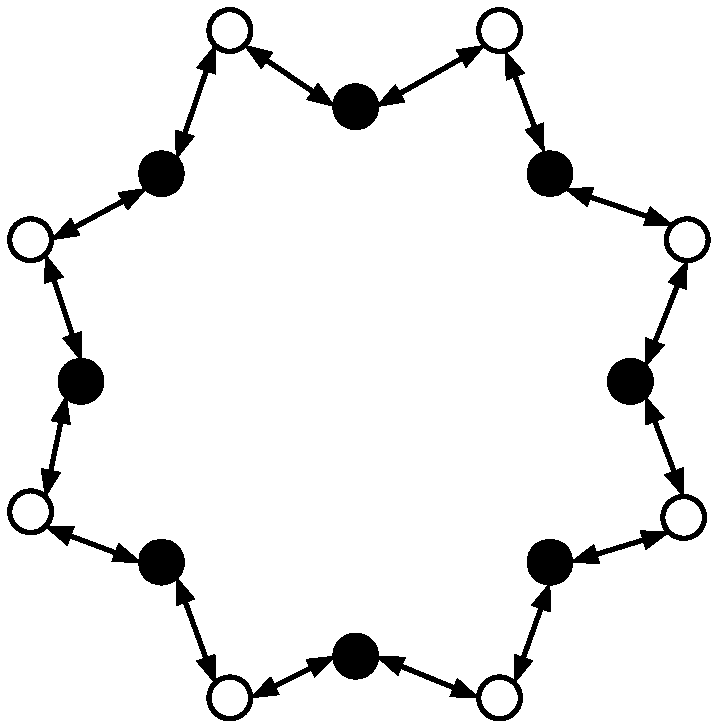
\includegraphics[scale=0.4]{PRing.pdf}
    \end{figure}
    \note{Reference Slide.}
\end{slide}

\begin{slide}
\frametitle{Results: Longevity-Based Batching}
{\scriptsize
\begin{table}
    \centering
    \begin{tabular}{ccccc} & \multicolumn{4}{c}{ $PTree_{(4,8)}$ } \\ \cline{2-5}
    \multicolumn{1}{c}{\textbf{Time}} & \multicolumn{2}{c}{ $MTRRWS$-$SQ$ } & \multicolumn{2}{c}{ Long. Batcher} \\ \cline{2-5}
    \multicolumn{1}{c|}{\textbf{Quantum}} & \textbf{Chan. State} & \multicolumn{1}{c|}{\textbf{Reduc. Density}} 
                                                & \textbf{Chan. State} & \multicolumn{1}{c|}{\textbf{Reduc. Density}} \\ \cline{1-5}
    \multicolumn{1}{c|}{$R=30$} &  \multicolumn{1}{c}{\includegraphics[scale=0.11]{tests/ptree/wssq/ca30r/pg_0003.pdf}} &
                                   \multicolumn{1}{c|}{\includegraphics[scale=0.11]{tests/ptree/wssq/ca30r/pg_0004.pdf}} &
                                   \multicolumn{1}{c}{\includegraphics[scale=0.11]{tests/ptree/lbb/ca30r/pg_0003.pdf}} &
                                   \multicolumn{1}{c|}{\includegraphics[scale=0.11]{tests/ptree/lbb/ca30r/pg_0004.pdf}} \\ \cline{1-5}

%    \multicolumn{1}{c|}{$R=40$} &  \multicolumn{1}{c}{\includegraphics[scale=0.1]{tests/ptree/wssq/ca40r/pg_0003.pdf}} &
%                                   \multicolumn{1}{c|}{\includegraphics[scale=0.1]{tests/ptree/wssq/ca40r/pg_0004.pdf}} &
%                                   \multicolumn{1}{c}{\includegraphics[scale=0.1]{tests/ptree/lbb/ca40r/pg_0003.pdf}} &
%                                   \multicolumn{1}{c|}{\includegraphics[scale=0.1]{tests/ptree/lbb/ca40r/pg_0004.pdf}} \\ \cline{1-5}

    \multicolumn{1}{c|}{$R=50$} &  \multicolumn{1}{c}{\includegraphics[scale=0.11]{tests/ptree/wssq/ca50r/pg_0003.pdf}} &
                                   \multicolumn{1}{c|}{\includegraphics[scale=0.11]{tests/ptree/wssq/ca50r/pg_0004.pdf}} &
                                   \multicolumn{1}{c}{\includegraphics[scale=0.11]{tests/ptree/lbb/ca50r/pg_0003.pdf}} &
                                   \multicolumn{1}{c|}{\includegraphics[scale=0.11]{tests/ptree/lbb/ca50r/pg_0004.pdf}} \\ \cline{1-5}
    \end{tabular}
\end{table}
}
    \inote{
        \item Comparison of $PTree_{(4,8)}$ running with the Longevity-Based 
        Batching Scheduler and $MTRRWS$-$SQ$ at different time-quantums.

        \item Absorption channels help here to relocate processes.

        \item At lower time quantums Long. Batcher starts to look like RRWS-SQ, 
            however batching and absorption channels tend to lead to consolidation.

        \item At higher time quantums Long. Batcher results in the originally expected
            work-groups. But it turns out to be inefficient due to lost chances of
            parallelism of each "star" of each group.

        \item Heuristical adjustment of the time-quantum would definitely be possible.

        \item NOTE: We don't capture overhead of stealing. Batching has obvious gains here.
    }
\end{slide}

\begin{slide} % FOR READERS
    \begin{figure}
        \centering
        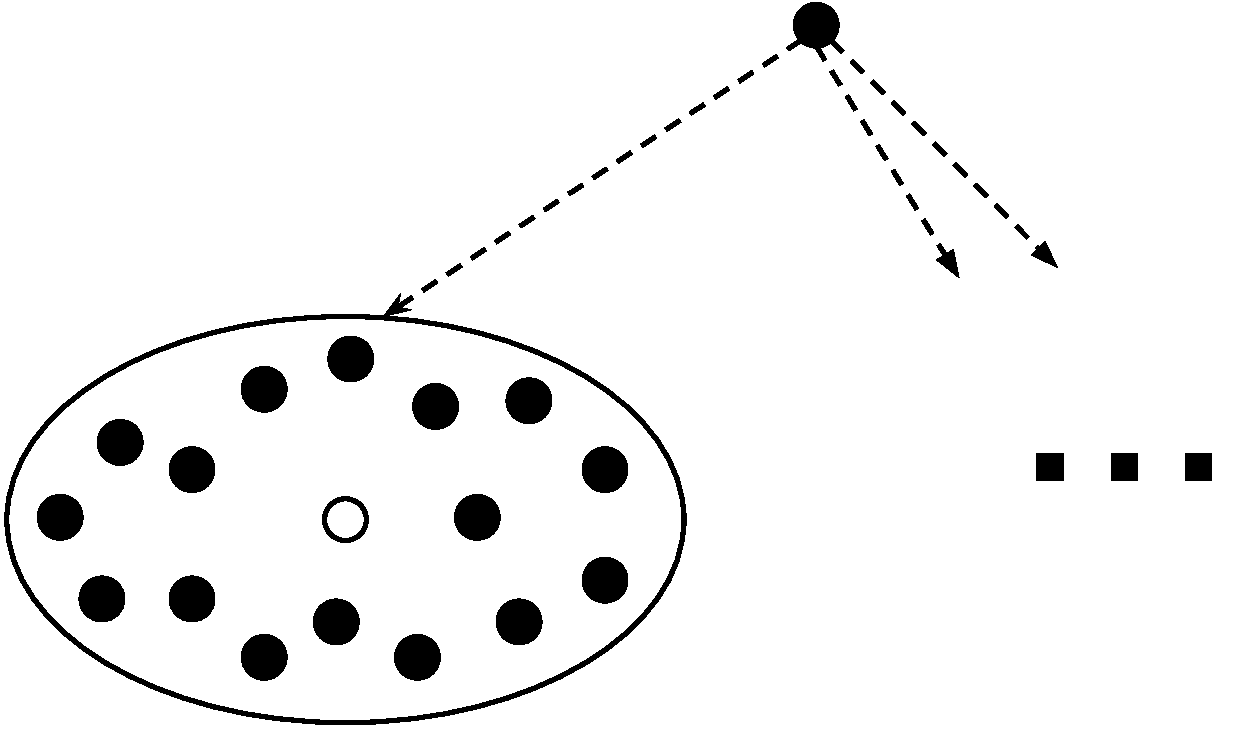
\includegraphics[scale=0.4]{PTree.pdf}
    \end{figure}
    \note{Reference Slide.}
\end{slide}

\begin{slide}
\frametitle{Results: Channel Pinning}
    \begin{table}
    \centering
    \begin{tabular}{@{}ccc}
    & \multicolumn{2}{c}{$Interactivity_{(20,0)}$} \\ \cline{2-3} 
    & \multicolumn{1}{c}{$MTRRWS$-$SQ$}       & \multicolumn{1}{c}{Channel Pinning} \\ \cline{2-3} 
 
    \multicolumn{1}{c|}{\rotatebox{90}{\rlap{~~Queue Length}}} &
    \multicolumn{1}{c}{\includegraphics[scale=0.15]{tests/interactivity/20/wssq/ca/pg_0003.pdf}} & 
    \multicolumn{1}{c|}{\includegraphics[scale=0.15]{tests/interactivity/20/cp/ca/pg_0003.pdf}} \\

    \multicolumn{1}{c|}{\rotatebox{90}{\rlap{Reduc. Density}}} &
    \multicolumn{1}{c}{\includegraphics[scale=0.15]{tests/interactivity/20/wssq/ca/pg_0004.pdf}} & 
    \multicolumn{1}{c|}{\includegraphics[scale=0.15]{tests/interactivity/20/cp/ca/pg_0004.pdf}} \\ \cline{2-3}
    \end{tabular}
    \label{tab:cp-compare-rand-uniform-ca}
    \end{table}

    \inote{
        \item Comparison of Uniform synchronization for $MTRRWS$-$SQ$ 
                and the Channel Pinning Scheduler on Absorption Channels.
        \item This used the $even$ spread type.
        \item Note the speed at which it saturates all cores.
        \item Despite Naive WS, we still have decent spread.
    }
\end{slide}


\begin{slide} % FOR READERS
    \begin{figure}
        \centering
        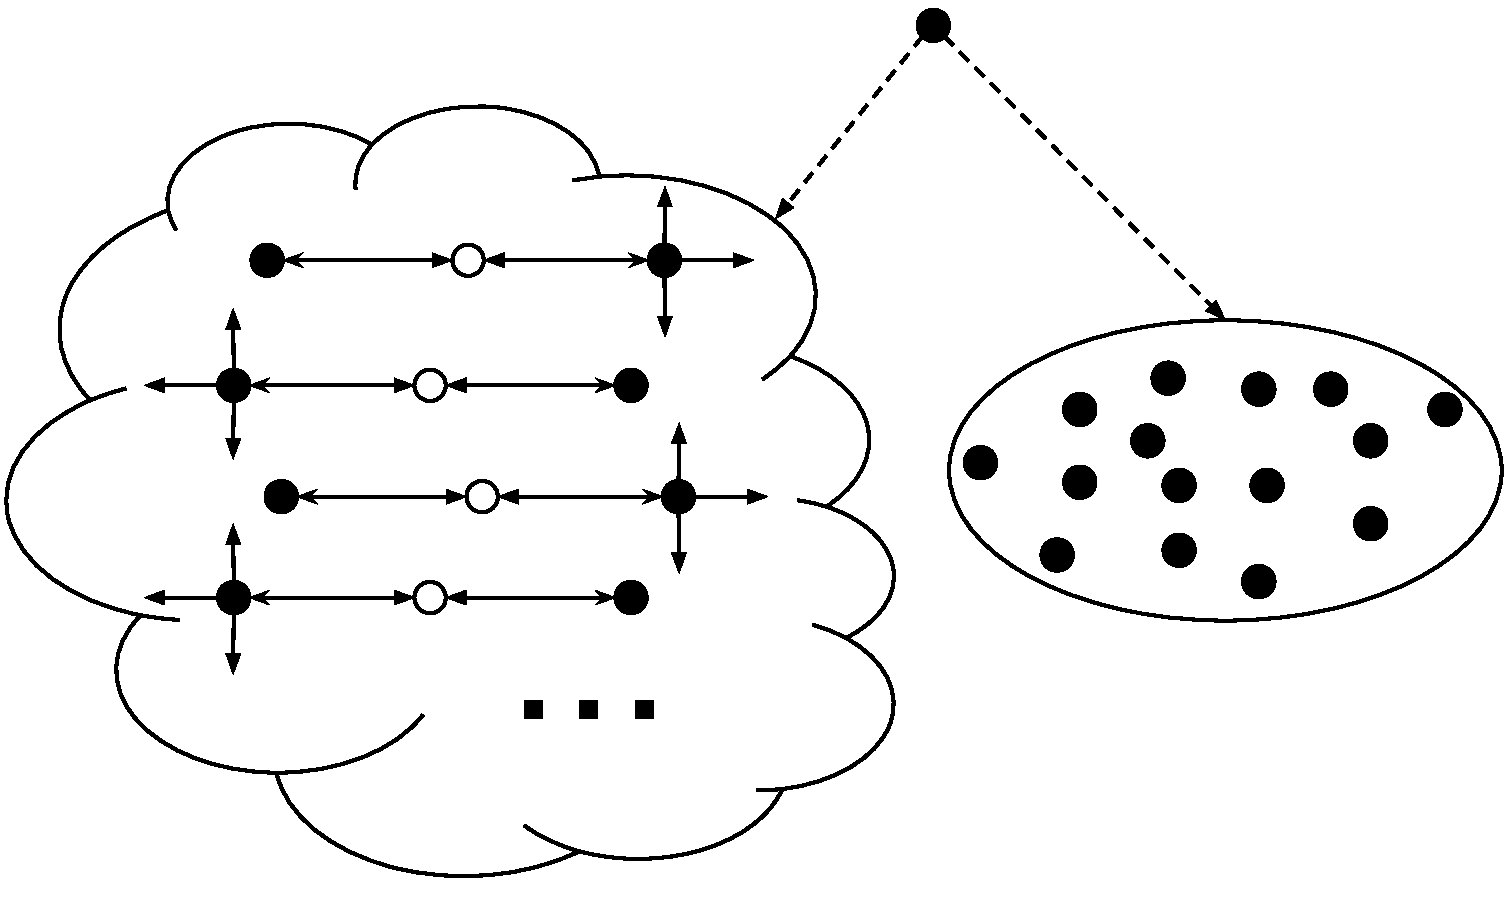
\includegraphics[scale=0.4]{Interactivity.pdf}
    \end{figure}
    \note{Reference Slide.}
\end{slide}

\begin{slide}
    \framesubtitle{Results: Bipartite-Aided Graph Sorting}
    \begin{figure}
        \centering
        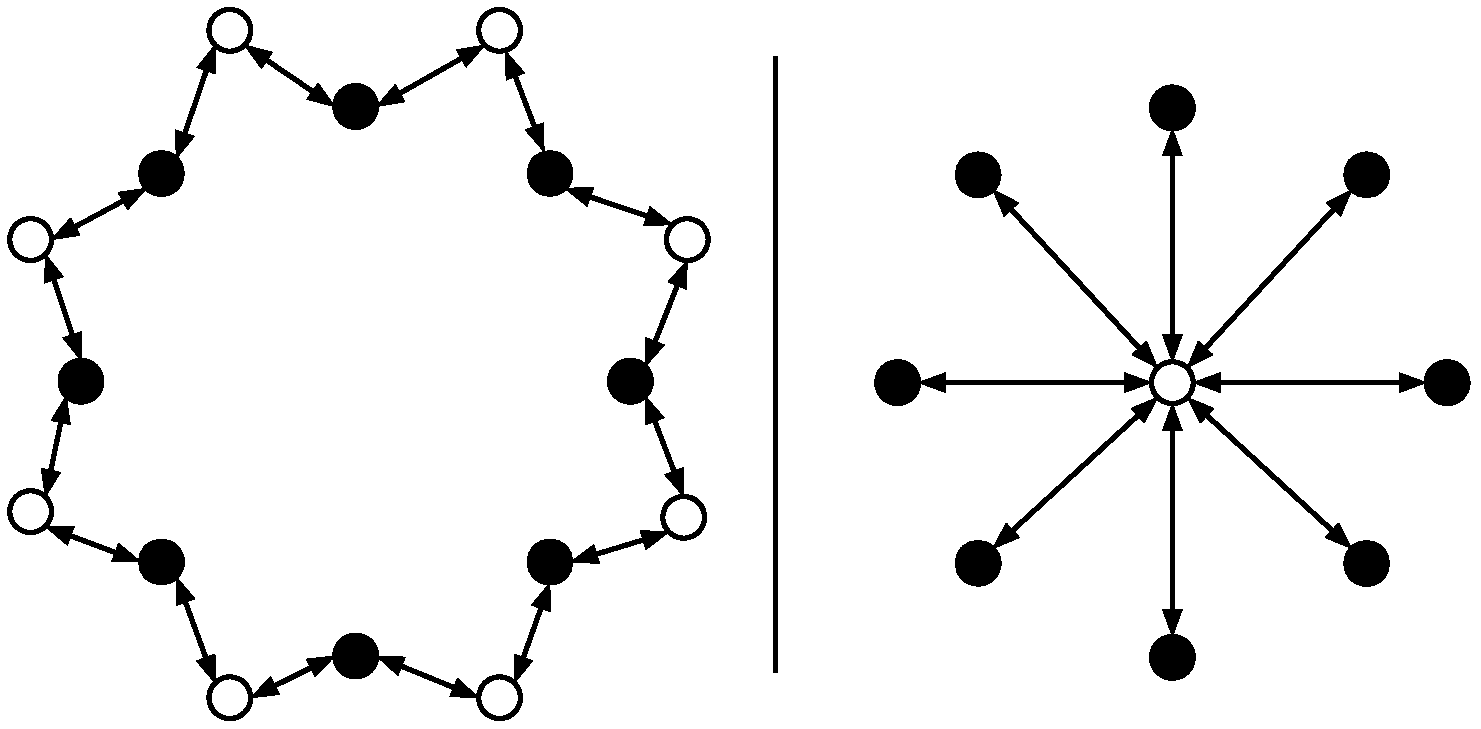
\includegraphics[scale=0.4]{RingVCluster.pdf}
    \end{figure}

    \inote{
        \item There is an issue with our next test.
        \item Our base primitive behaviours don't have a preferred order of
            execution.
        \item Ring does, but there is nothing parallel about it.
    }

\end{slide}

\begin{SaveVerbatim}[commandchars=\\\{\}]{FibCode}
fun N.
    (omega \textbf{fun} f,m.(
        \textbf{if} (leq m 1) 
           m
           (merge \textbf{fun} _.(f f (sub m 1))
                  \textbf{fun} _.(f f (sub m 2))
                  add)) \textit{N})
\end{SaveVerbatim}
\begin{slide}
    \framesubtitle{Results: Bipartite-Aided Graph Sorting}
    \begin{figure}
        \centering
        {\small
            \BUseVerbatim{FibCode}
        } 
    \end{figure}
    
    \inote{
        \item We therefore used a parallel Fibonacci program.
        \item Merge function waits for each sub process to finish before
                running Add.
        \item If we sort based on who hasn't had a chance to communicate yet,
            we can preferentialize these MapReduce style applications, while
            not decrementing possible execution in parents.
    }
\end{slide}

\begin{slide}
\frametitle{Results: Bipartite-Aided Graph Sorting}

    \begin{table}
    \centering
    \begin{tabular}{@{}ccc}
        & \multicolumn{2}{c}{Parallel Fibonacci} \\ \cline{2-3}
        & $MTRRWS$-$SQ$ & Sorting Scheduler  \\ \cline{2-3} 
        \multicolumn{1}{c|}{~}  & 
        \multicolumn{1}{c|}{\includegraphics[scale=0.27]{tests/pfib/wssq/pg_0001.pdf}} & 
        \multicolumn{1}{c|}{\includegraphics[scale=0.27]{tests/pfib/ss/pg_0001.pdf}} \\ \cline{2-3}
    \end{tabular}
    \label{tab:ss-compare-fib}
    \end{table}

    \inote{
        \item PFib has a strong reliance on order of execution.
        \item Channel State comparison of Parallel Fibonacci executed on 
                $MTRRWS$-$SQ$ and the Bipartite-Graph Aided Sorting Scheduler. 
        \item Note the large reduction in number of ticks.
    }
\end{slide}

